%% March 2018
%%%%%%%%%%%%%%%%%%%%%%%%%%%%%%%%%%%%%%%%%%%%%%%%%%%%%%%%%%%%%%%%%%%%%%%%%%%%
% AGUJournalTemplate.tex: this template file is for articles formatted with LaTeX
%
% This file includes commands and instructions
% given in the order necessary to produce a final output that will
% satisfy AGU requirements, including customized APA reference formatting.
%
% You may copy this file and give it your
% article name, and enter your text.
%
%%%%%%%%%%%%%%%%%%%%%%%%%%%%%%%%%%%%%%%%%%%%%%%%%%%%%%%%%%%%%%%%%%%%%%%%%%%%
% PLEASE DO NOT USE YOUR OWN MACROS
% DO NOT USE \newcommand, \renewcommand, or \def, etc.
%
% FOR FIGURES, DO NOT USE \psfrag or \subfigure.
% DO NOT USE \psfrag or \subfigure commands.
%%%%%%%%%%%%%%%%%%%%%%%%%%%%%%%%%%%%%%%%%%%%%%%%%%%%%%%%%%%%%%%%%%%%%%%%%%%%
%
% Step 1: Set the \documentclass
%
% There are two options for article format:
%
% PLEASE USE THE DRAFT OPTION TO SUBMIT YOUR PAPERS.
% The draft option produces double spaced output.
%

%% To submit your paper:
%\documentclass[draft,linenumbers]{agujournal2018}  %%%%%%%%%%switch this back for linenumbers
%\documentclass[draft]{agujournal2018}
%\usepackage{apacite}
%\usepackage{url} %this package should fix any errors with URLs in refs.

\documentclass[main.tex]{subfiles}


%%%%%%%
% \usepackage{trackchanges}
% uncomment the line above to use the TrackChanges package to mark revisions if needed.
% The trackchanges package adds five new LaTeX commands:
%
%  \note[editor]{The note}
%  \annote[editor]{Text to annotate}{The note}
%  \add[editor]{Text to add}
%  \remove[editor]{Text to remove}
%  \change[editor]{Text to remove}{Text to add}
%
% complete documentation is here: http://trackchanges.sourceforge.net/
%%%%%%%

%\draftfalse

% Now, type in the journal name: \journalname{<Journal Name>}

% ie, \journalname{Journal of Geophysical Research}
%% Choose from this list of Journals:
%
% JGR-Atmospheres
% JGR-Biogeosciences
% JGR-Earth Surface
% JGR-Oceans
% JGR-Planets
% JGR-Solid Earth
% JGR-Space Physics
% Global Biochemical Cycles
% Geophysical Research Letters
% Paleoceanography
% Radio Science
% Reviews of Geophysics
% Tectonics
% Space Weather
% Water Resource Research
% Geochemistry, Geophysics, Geosystems
% Journal of Advances in Modeling Earth Systems (JAMES)
% Earth's Future
% Earth and Space Science
% Geohealth
%

%\journalname{Journal of Geophysical Research}


\begin{document}

%% ------------------------------------------------------------------------ %%
%  Title
%
% (A title should be specific, informative, and brief. Use
% abbreviations only if they are defined in the abstract. Titles that
% start with general keywords then specific terms are optimized in
% searches)
%
%% ------------------------------------------------------------------------ %%

% Example: \title{This is a test title}

%\title{Low Temperature Plastic Deformation of Confined Olivine With Free Surfaces}

%% ------------------------------------------------------------------------ %%
%
%  AUTHORS AND AFFILIATIONS
%
%% ------------------------------------------------------------------------ %%

% Authors are individuals who have significantly contributed to the
% research and preparation of the article. Group authors are allowed, if
% each author in the group is separately identified in an appendix.)

% List authors by first name or initial followed by last name and
% separated by commas. Use \affil{} to number affiliations, and
% \thanks{} for author notes.
% Additional author notes should be indicated with \thanks{} (for
% example, for current addresses).

% Example: \authors{A. B. Author\affil{1}\thanks{Current address, Antartica}, B. C. Author\affil{2,3}, and D. E.
% Author\affil{3,4}\thanks{Also funded by Monsanto.}

\authors{Eric Burdette, Cameron Meyers, and Greg Hirth}


%\affiliation{1}{Brown University}
% \affiliation{2}{Second Affiliation}
% \affiliation{3}{Third Affiliation}
% \affiliation{4}{Fourth Affiliation}

\affiliation{1}{Department of Earth, Environmental and Planetary Sciences, Brown University, Providence, RI, USA}
%(repeat as many times as is necessary)

%% Corresponding Author:
% Corresponding author mailing address and e-mail address:

% (include name and email addresses of the corresponding author.  More
% than one corresponding author is allowed in this LaTeX file and for
% publication; but only one corresponding author is allowed in our
% editorial system.)

% Example: \correspondingauthor{First and Last Name}{email@address.edu}

%\correspondingauthor{Eric Burdette}{eric\_burdette@brown.edu}

%% Keypoints, final entry on title page.

% Example:
% \begin{keypoints}
% \item	List up to three key points (at least one is required)
% \item	Key Points summarize the main points and conclusions of the article
% \item	Each must be 100 characters or less with no special characters or punctuation
% \end{keypoints}

%  List up to three key points (at least one is required)
%  Key Points summarize the main points and conclusions of the article
%  Each must be 100 characters or less with no special characters or punctuation

\begin{keypoints}
    \item Porosity-free sintered olivine pillars were deformed at stresses up to 4 GPa at room temperature and 600°C.
    \item Kinks dominate surface microstructure, with many tightly spaced bands in optimally oriented bands.
\end{keypoints}

\clearpage
%% ------------------------------------------------------------------------ %%
%
%  ABSTRACT
%
% A good abstract will begin with a short description of the problem
% being addressed, briefly describe the new data or analyses, then
% briefly states the main conclusion(s) and how they are supported and
% uncertainties.
%% ------------------------------------------------------------------------ %%

%% \begin{abstract} starts the second page

% \begin{abstract}
% ??? Placeholder
% \end{abstract}



%% ------------------------------------------------------------------------ %%
%
%  TEXT
%
%% ------------------------------------------------------------------------ %%


\section{Introduction}
    To understand the spatial and temporal distribution of earthquakes in the mantle lithosphere, as well as the processes responsible for the wide spectrum of fault slip behaviors, it is important to constrain rheological properties of olivine aggregates. Seismicity in the oceanic lithosphere is generally limited to depths at which the temperature is less than approximately 600°C. Seismic behavior is possible when the friction coefficient decreases with increasing sliding velocity (i.e., velocity weakening behavior characterized by rate-and-state friction). Laboratory studies on olivine friction at low normal stress demonstrate a transition from velocity weakening to velocity strengthening with an increase in temperature from 800 to 1000°C \citep{boettcher2007olivine, king2012frictional}. Recent analyses of mantle fault rocks from oceanic transform faults provides evidence of fluid penetration facilitated by brittle deformation at temperatures up to ~900°C – consistent with observations of seismicity in the mantle at transform faults at similar temperatures \citep{kuna2019mode, mcguire2012rogue, roland2012seismic}. These observations have motivated analyses highlighting the importance of strain rate and temperature on lithosphere rheology near the brittle-plastic transition \citep[e.g.][]{molnar2020brittle}.
    
    A fundamental issue related to this problem is the magnitude of stresses supported by  the mantle lithosphere near the brittle-plastic transition. Comparisons of geophysical data with geodynamic models suggest stresses do not exceed ~300 MPa, a value far less than predicted by applying standard friction laws at the depth limit of seismicity (e.g., Kohlstedt et al., 1995). At these conditions, olivine aggregates are generally interpreted to deform by low-temperature plasticity (sometimes called Peierls creep) – a process that is rate-limited by dislocation glide. Laboratory tests and theory indicate that the yield strength for dislocation glide is considerably lower than the steady-state flow stress \citep[e.g.][]{idrissi2016low, hansen2019low}, leading to more sophisticated analyses of strain hardening and grain-size effects (i.e. Hall-Petch) on dislocation glide in olivine. By accounting for these factors, the extrapolation of lab data can align with the geodynamic constraints for the stress magnitude if one considers low strain (i.e., prior to significant strain hardening) and low strain rate deformation \citep[e.g.][]{hansen2019low}. However, this data is collected in relatively short times, making extrapolation uncertainty large, and recovered samples do not preserve microstructure and deformation mechanisms that lead to proposed strain hardening and laws.
    
    To better constrain low temperature plasticity mechanisms in olivine, we developed a new Griggs-apparatus assembly to deform strong pillars in hydraulic oil and loose graphite confining media which preserve pre-polished sample surfaces. The recovered samples illustrate activity of orientation-dependent kinking and grain interactions which is discussed below.

\section{Materials and Methods}

    \subsection{Materials}
        The samples used in our preliminary work were synthesized by evacuated hot pressing powdered San Carlos olivine in a Paterson-type gas-medium apparatus at 1250 °C and 300 MPa confining pressure. Active evacuation of the pore spaces leads to samples with <0.0001 porosity (Meyers et al., 2017, AGU abstract), such that they have high fracture toughness, enabling low-temperature plasticity at high confining pressures.
        Mean grain size is 10 $\mu$m.
        
        Multiple rectangular pillars are cut from a single cylindrical hot-pressed sample. They are then squared and polished to 0.1 $\mu$m surface finish with diamond lapping paper. 
        
    \subsection{Methods}
        Two new cell assemblies were designed for this work. The first relies on BUNA rubber seals to contain hydraulic oil inside the pressure vessel at room temperature (Figure \ref{fig:A2_AssembliesRT}). Alignment of the pistons and sample are critical for even stress application so several additional elements are included which are not needed for typical oil-confined assemblies. 
        
        \begin{figure}
          \includegraphics[width=\textwidth]{Figures/Pillar Assembly1_biglabels.pdf}
          \caption{Schematic of Modified assembly for olivine pillar deformation at room temperature}
          \label{fig:A2_AssembliesRT}
        \end{figure}
        
        The second assembly adapts a standard assembly used for high temperature (600°C) creep tests by placing the sample pillar between alumina pistons inside an annealed brass sleeve. The sleeve has a drilled round hole whose diameter is slightly larger than the corner-to-corner distance of the pillar placed inside it. The space between the pillar and the sleeve is filled with loose graphite powder and the entire brass capsule is placed inside a standard annealed silver jacket. The brass prevents pre-loading of the sample during pressurization and anneals/weakens at high temperature to apply confining pressure and allow deformation of the sample. The brass jacket protects potentially brittle samples during decompression. The jacket is ground/machined off after deformation, and the pillar surfaces are protected by the graphite powder which can be brushed off.
        
        Stress and displacement are determined using the methods described in Matej Pec's Rig 1.3 program (https://sites.google.com/site/rigprogram/home) and constant stress deformation methods described in Chapter 2.

\section{Results}
    \subsection{Mechanical Results}
        Broadly our results agree with \citet{hansen2019low}.  We record yielding at ~2.4 GPa at room temperature, and strength at 600°C similar to that recorded by \citet{hansen2019low} (Figure \ref{fig:A2_Druiventak}). At 2.25 GPa pressure samples are clearly less brittle, yielding and hardening for much longer than the fracture at 1 GPa (Figure \ref{fig:A2_ConstStrainrateRT}). In all cases the samples approach brittle failure, with microcracks decorating grain boundaries (Figure \ref{fig:A2_OpticalKinks}). Our results are significantly stronger than \citet{druiventak2011low}, likely because natural dunites contain alteration phases at grains boundaries which could weaken them.
        
        \begin{figure}
          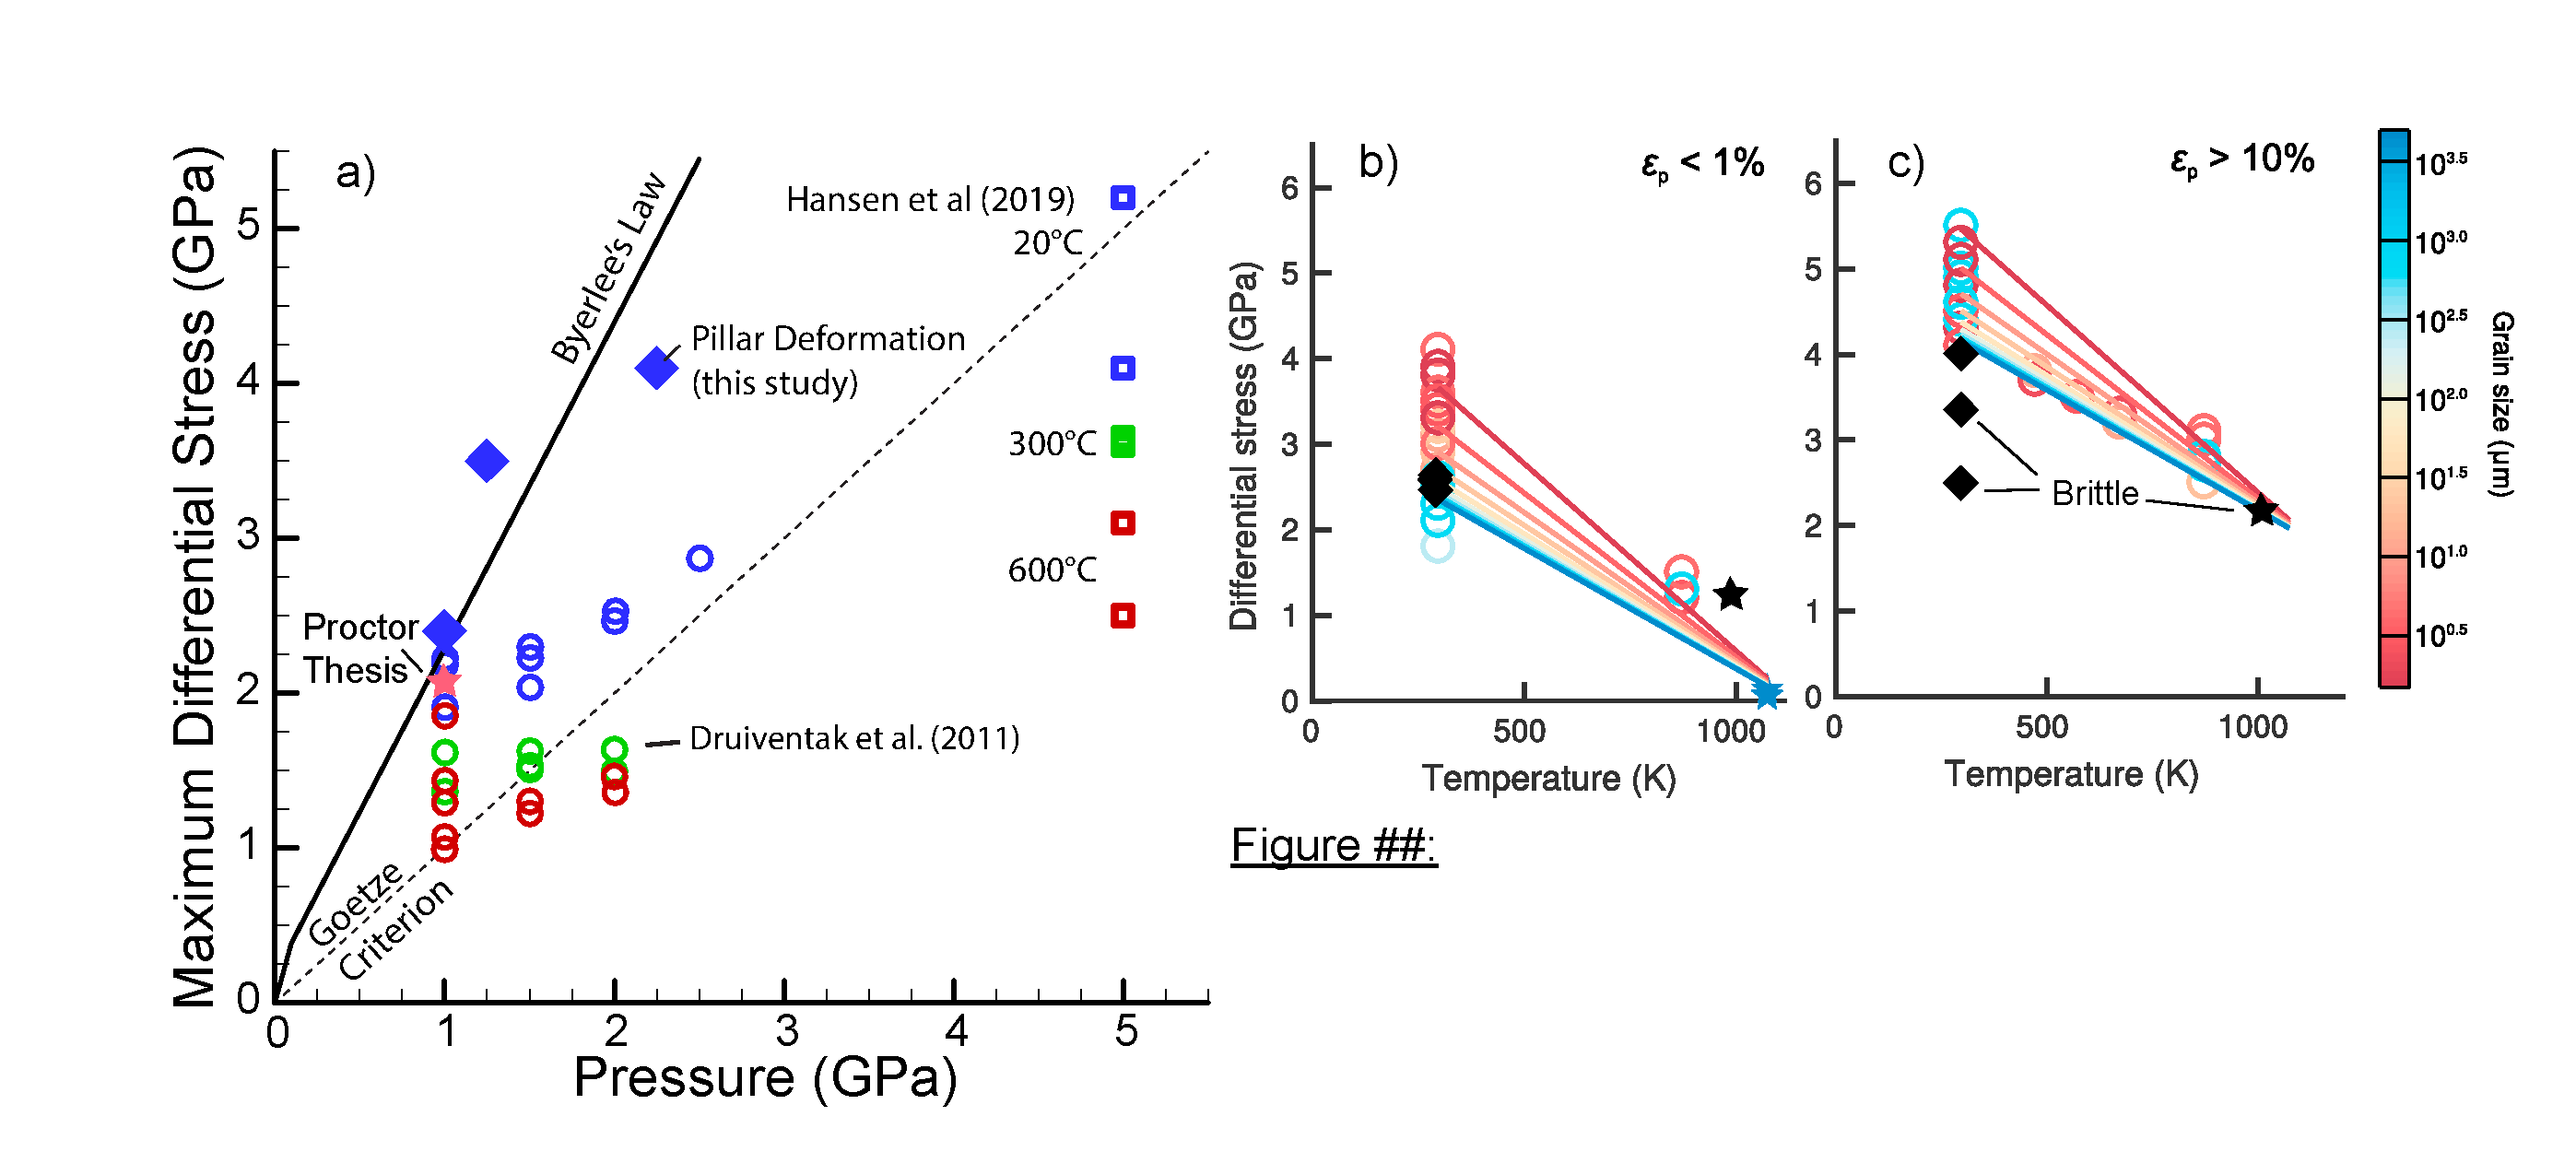
\includegraphics[width=\textwidth]{Figures/Druiventaketal_datasets_summary+yield2.pdf}
          \caption{Strength and yield data for olivine deformation. Diamonds are pillar experiments, star is  published in the thesis of Brooks Proctor. a) is colored by temperature.}
          \label{fig:A2_Druiventak}
        \end{figure}
        
        \begin{figure}
          \includegraphics[width=\textwidth]{Figures/Ol_PillarMechDataRT.png}
          \caption{Room temperature deformation data for two olivine pillars}
          \label{fig:A2_ConstStrainrateRT}
        \end{figure}
        
        \begin{figure}
          \includegraphics[width=\textwidth]{Figures/Olivine_optical_kinks_Cam.png}
          \caption{Optical image of olivine surface recovered after room temperature deformation. Cracks are common along grain boundaries, and optical topography contrast is due to misorientation of kink bands to the surrounding surface. Compression direction is vertical.}
          \label{fig:A2_OpticalKinks}
        \end{figure}
                
    \subsection{Microstructure}
        Because samples were initially lapped below 0.1 um roughness with colloidal silica, so optically visible changes represent changes in surface topography induced by deformation. Samples were characterized optically first (Figure \ref{fig:A2_OpticalKinks}). The images show light and dark bands throughout single grains. The bands are mostly oriented perpendicular to the axial compression direction. Cracks are prevalent throughout the images, found almost exclusively along grain boundaries.
        Grains were also characterized with a Brukers AXS atomic force microscope and ultrasharp contact tips. The images show 'steps' at a smaller scale than was optically visible (Figure \ref{fig:A2_AFMmap}). A transect perpendicular to the bands (Figure \ref{fig:A2_AFMProfile}) shows the existence of sharp corners on these steps, and similar angles throughout the set of about 5 degrees. Some of these steps are on the order of 1 nm potentially constituting single slip bands.
        
        \begin{figure}
          \includegraphics[width=\textwidth]{Figures/AFM_image2516_1.png}
          \caption{AFM image of a deformed grainwith stepwise kink bands. Many small features are visible that cannot be resolved optically.}
          \label{fig:A2_AFMmap}
        \end{figure}
        
        \begin{figure}
          \includegraphics[width=\textwidth]{Figures/Annotated_kink_profile.png}
          \caption{Profile along transect perpendicular to kink bands in Figure \ref{fig:A2_AFMmap}. Topography is exaggerated, and steps as small as 1 nm are resolved in the trace.}
          \label{fig:A2_AFMProfile}
        \end{figure}

        
        
\section{Discussion}
    \subsection{Kinks}
        Nucleation of pairs of dislocations in the direction of axial compression could form dipole pairs which expand until they reach the edges of the sample and form kinks (Figure \ref{fig:A2_StepwiseKink}). The low angles we record in AFM support this hypothesis, although EBSD and TEM will be needed to characterize dislocation density variation with depth to verify the model.
        
        \begin{figure}
          \includegraphics[width=\textwidth]{Figures/Stepwise_kinking_Diagram.png}
          \caption{Diagram showing schematically ho kinks produce the surface topography }
          \label{fig:A2_StepwiseKink}
        \end{figure}
        
    \subsection{Mechanical strength}
        These experiments show that even at room temperature, olivine can deform by dislocation motion in polycrystalline samples. The observed deformation is clearly strongly orientation dependent, which could pose problems for extrapolating single-crystal mechanisms to polycrystalline samples. We plan to continue examining hardening and long-term creep rate in future studies.
    

\section{Conclusions}
        Here we deformed vacuum-sintered olivine at room temperature and 600°C in novel assemblies to preserve surface features. The samples had strengths similar to\citet{hansen2019low}, and show a clear surface pattern indicating orientation-dependent kinking was active.
    
    \begin{enumerate}
        \item Kink bands dominate room temperature deformation in olivine.
        \item Small features on the order of one burgers vector are present on the surface, possibly representing the termination of single-dislocation slip bands.
        \item Features are strongly orientation dependent, suggesting activation of a single slip system in olivine.
    \end{enumerate}

%Text here ===>>>
\acknowledgments
We would like to thank Lars Hansen for helpful discussions.

%\bibliography{Feb19_refs_2.bib}

\clearpage

\end{document}